\chapter{On Simulink}\label{App:Simulink}

\section{Model Linearizer Tools}\label{App:Simulink:ModelLinearizer}
The model linearizer tools is an ``App'' in Simulink that allows an engineer to
(1) linearize a system and (2) perform linear system analyses such as Bode
plots and Step Responses. We won't be needing the first feature since our
systems are already linear. This section is a brief tutorial on how to use
the tools to acquire step responses, Bode plots and Nyquist plots.

\subsection{The Model Linearizer App}
To open the Model Linearizer App, look to the top of your Simulink Model
window and click the ``\texttt{APPS}'' button like so
%
\begin{center}
  \includegraphics[width=0.8\linewidth]{%
    app-model-linearizer-open-1.png%
  }
\end{center}
%
Then proceed to opening the application by clicking the ``\texttt{Model
Linearizer}'' button
%
\begin{center}
  \includegraphics[width=0.8\linewidth]{%
    app-model-linearizer-open-2a.png%
  }
\end{center}
%
If you cannot find it located in the toolbar depicted above, press the
dropdown on the far right of the toolbar
%
\begin{center}
  \includegraphics[width=0.8\linewidth]{%
    app-model-linearizer-open-2b.png%
  }
\end{center}
%
to view a larger list of options.
If you still cannot find it, you must not have the \texttt{Simulink Control Design} toolbox installed. Ensure you've installed the toolboxes listed in the
Introduction. Upon opening the Model Linearizer app, you
will have a window that looks like Figure~\ref{fig:app1:model-linearizer}.
%
\begin{figure}[H]
  \centering
  \includegraphics[width=0.8\linewidth]{%
    app-model-linearizer-opened.png%
  }
  \caption[The Model Linearizer App]{%
    What the Model Linearizer application looks like when you first open it.%
  }
  \label{fig:app1:model-linearizer}
\end{figure}

\subsection{Setting up your System: Input to Output}
\label{App:Simulink:ModelLinearizer:2}
Now that you know how to open up the Model Linearizer, we must prepare
the system we want to analyze. The Model Linearizer tool doesn't know what
we consider an ``input'' and what we consider an ``output'' just from our
Simulink diagram. But you do! Whenever you want to take a step response, you
know where you input the step and what measurements you want to observe.
The goal of the following steps is to show you how to give the Model
Linearizer App this information.

First pull up the Simulink model of concern. I'll use the Lab 1 diagram as
an example,
%
\begin{center}
  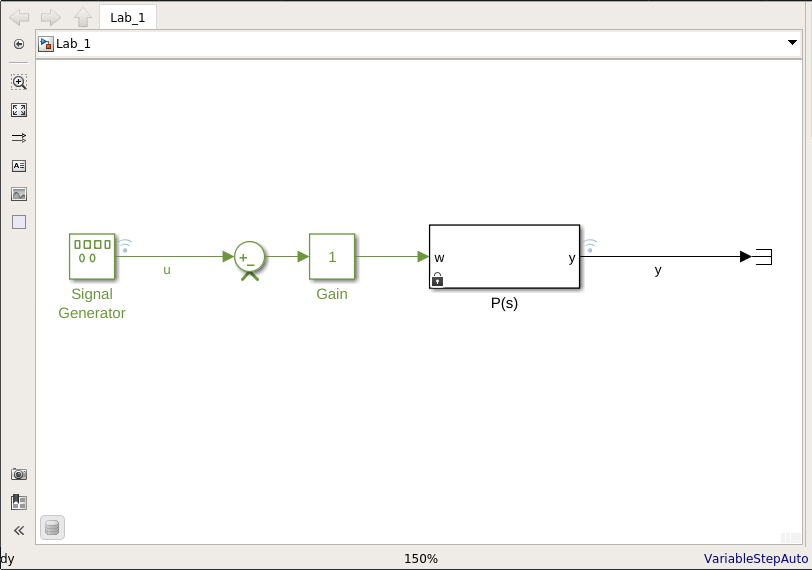
\includegraphics[width=0.8\linewidth]{app-model-linearizer-io-1.png}
\end{center}
%
Suppose we wanted to analyze the relationship between the signals
labelled \(u\) and \(y.\)
Right-click the signal wire labelled \(u\) and hover over ``Linear Analysis
Points'' as depicted in Figure~\ref{fig:app1:io-menu:a}.
%
\begin{figure}
  \centering
  \includegraphics[width=0.8\linewidth]{%
    app-model-linearizer-io-2a.png%
  }
  \caption{Signal context menu and Linear Analysis points submenu.}
  \label{fig:app1:io-menu:a}
\end{figure}
%
\begin{figure}
  \centering
  \includegraphics[width=0.8\linewidth]{%
    app-model-linearizer-io-2b.png%
  }
  \caption{The Linear Analysis context submenu.}
  \label{fig:app1:io-menu:b}
\end{figure}
%
This context menu has a number of options of which we will only use two.
Since we would like to indicate to the Model Linearizer App that this wire
is where the input appears, we select ``\texttt{Input Perturbation}.'' We
repeat the \emph{same exact} process for the desired output signal wire \(y\)
except we select ``\texttt{Output Measurement}.'' The result is
depicted in Figure~\ref{fig:app1:io-signals}. \emph{Note the little annotations
above the signal.}
A ``down'' arrow denotes an input and an ``up'' arrow denotes an output signal.
%
\begin{figure}
  \centering
  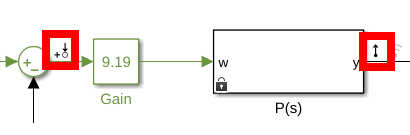
\includegraphics[width=0.8\linewidth]{app-model-linearizer-io-3.png}
  \caption{%
    The result after setting up an input signal and output
    measurement signal.%
  }
  \label{fig:app1:io-signals}
\end{figure}
%
You will have to repeat this process whenever you want to change where you
apply your input or when you want to observe a different output. Note that
the placement of the ``\texttt{Input Perturbation}'' and
``\texttt{Output Measurement}'' annotations is not arbitrary;
it is intentional! This
allows us to quickly change the configuration of the system, closing the loop
for example, and get closed-loop measurements without having to change our
annotations!

\FloatBarrier
\subsection{Acquiring Plots}
\label{App:Simulink:ModelLinearizer:3}
Having indicated to the Model Linearizer app the input and output signal, you
are now ready to acquire a step response. Open the Model Linearizer. Look at
the top bar of the Model Linearizer and confirm that it looks as depicted below:
%
\begin{center}
  \includegraphics[width=0.8\linewidth]{%
    app-model-linearizer-toolbar.png%
  }
\end{center}
%
Try pressing the ``\texttt{Step Response}'' button! You should get a response
like that of Figure~\ref{fig:app1:stepresponse}. Great! Now try clicking
on a point of the curve. You will then get something we call a \textbf{data
tip} or \textbf{cursor}, shown in Figure~\ref{fig:app1:cursors}.
You can drag this cursor (the black dot) around to a specific point on the
curve, allowing you to get accurate readings. Use this feature!
%
Similarly, one can capture a Bode plot, as depicted in Figure
\ref{fig:app1:bodeplot}, by pressing the ``\texttt{Bode}'' button.

Now that we can acquire these plots, how do we \emph{save} them? Notice that
above every plot is a name. For example, Figure~\ref{fig:app1:bodeplot} is
in a tab named ``Bode Plot 1.'' With this selected, you will see in the top
bar a larger tab with the same name. This is depicted in Figure
\ref{fig:app1:capturefigure}. In that tab, you can then press
``\texttt{Print to Figure}.'' Upon doing so, you have a Matlab Figure pop-up,
which then gives you the option --- under \texttt{File/Save As} --- to
export a \texttt{.png} or other image file.
%
\begin{figure}
  \centering
  \includegraphics[width=0.8\linewidth]{%
    app-model-linearizer-stepresponse.png%
  }
  \caption[Capturing a Step Response in the Model Linearizer App]{%
    Capturing a step response in the Model Linearizer app.
  }
  \label{fig:app1:stepresponse}
\end{figure}
%
\begin{figure}
  \centering
  \includegraphics[width=0.8\linewidth]{%
    app-model-linearizer-cursors.png%
  }
  \caption[Data Tips in Matlab Figures]{%
    I put two data tips, one near the settling value and another at
    just over \(0.5\) in amplitude.
  }
  \label{fig:app1:cursors}
\end{figure}
%
\begin{figure}
  \centering
  \includegraphics[width=0.8\linewidth]{%
    app-model-linearizer-bodeplot.png%
  }
  \caption[Bode Plot captured in the Model Linearizer App]{%
    A bode plot captured in the Model Linearize app. Do you know what special
    points I've marked on the Bode plot? Name them. Why are they important?
  }
  \label{fig:app1:bodeplot}
\end{figure}
%
\begin{figure}
  \centering
  \includegraphics[width=0.8\linewidth]{%
    app-model-linearizer-capturefigure.png%
  }
  \caption[Acquiring a Figure in the Model Linearizer App]{%
    This screenshot depicts how to turn a data acquisition into a Matlab
    Figure.
  }
  \label{fig:app1:capturefigure}
\end{figure}
%
